\section{Lorentzian continuation and pole diagnostics}

We test the direct continuation
\begin{equation}
 z=-s-i0,\qquad s=(\omega^2-|\mathbf k|^2)/\Lam^2.\label{eq:cont}
\end{equation}
The entire quadratic functions have an unambiguous analytic extension, but this alone does not construct a causal quantum propagator or justify rotating a path integral through sectors of exponential growth. An integration contour, asymptotic state space, reflection positivity and ultraviolet unitarity remain separate questions. No alternate prescription is chosen to remove inconvenient zeros.

A simple real zero $z_*$ gives $s_*=-z_*$. Negative $z_*$ is timelike with positive squared mass parameter; positive $z_*$ is tachyonic under \eqref{eq:cont}. At a full neutral null vector $v$, normalized by $v_q^T\GE(0)v_q=1$,
\begin{equation}
 \KK^{-1}(z)=\frac{v v^T}{(z-z_*)v^T\KK'(z_*)v}+O(1),\qquad
 Z=\frac1{v^T\KK'(z_*)v}.\label{eq:residue}
\end{equation}
The real sign is compared with a healthy Euclidean kernel $z+m^2$. For the tensor it is the sign of $1/K_2'(z_*)$; we also quote its ratio to the massless residue, $f/[4K_2'(z_*)]$. At non-real zeros the transpose bilinear still gives the residue matrix, but a positive/negative norm sign is not defined. Matrix-inverse limits independently check the residues.

\subsection{An analytic tensor obstruction}

Let $\nu_a=w_aH_a/(16\pi^2a)>0$. The tensor form factor obeys
\begin{equation}
 \mathsf a(0)=f>0,\qquad
 K_2(z)\underset{z\to+\infty}{\longrightarrow}
 -\sum_a\frac{w_aH_a}{32\pi^2a^2}<0.\label{eq:tensorobstruction}
\end{equation}
The second statement follows from $F(x)=2/x+4/x^2+O(x^{-3})$ in \eqref{eq:aa}. Since $K_2(z)>0$ for small positive $z$, continuity forces at least one nonzero positive-real zero. This argument applies to the specified positive finite exponential sum and convergent internal heat traces, not merely to a finite momentum polynomial. It uses the total flat-stationary subtraction; retaining an uncanceled off-shell potential contact would change the expansion point.

Conversely, for $s\ge0$ each term of the timelike tensor factor has the series
\begin{equation}
 F(-as)-4J(-as)=
 \sum_{n=0}^{\infty}\frac{n!}{(2n+1)!}\frac{2n+1}{2n+3}(as)^n>0.\label{eq:positive}
\end{equation}
Thus $\mathsf a(-s)$ has no real timelike zero. The ordinary massless tensor pole remains, with positive slope $f/4$. The sign argument does not enumerate all spacelike or complex zeros or establish their residue signs; those are tested numerically below. Additional independent gravitational operators would change the conclusion and are not included here.

\subsection{Real poles on the four fixtures}

Within $-20\le z\le20$, the neutral coupled search finds four timelike poles and one positive-$z$ pole on each fixture. The three low-lying timelike poles connect to the two light neutral modes and the radion of the preceding derivative truncation. The fourth lies above the cutoff. The reported timelike squared parameters $s=-z$ are:

\begin{center}\small\TimelikeTable\end{center}

The radion-connected value at $\epsilon=0.01$, $f_-$ changes from $0.829596301$ in the two-derivative calculation to $0.656507988$, a roughly $20.9\%$ reduction in the squared parameter. The corresponding mass parameter changes from $0.91082\Lam$ to about $0.81025\Lam$. This comparison is internal to the retained operator; the same fixture has the instability below, so it is not a stable-particle prediction. The small light shifts and positive residues do not remove that obstruction.

\begin{center}\small\TachyonTable\end{center}

Here $z_T,z_S>0$ imply $s_T,s_S<0$. Both real zeros have negative residue signs. For the representative minus fixture, the tensor relative residue is approximately $-3.42635$. The neutral real-pole residues, using the normalization in \eqref{eq:residue}, are:
\begin{center}\small\ResidueTable\end{center}

The tachyonic scales are above $\Lam$, where an infrared-only effective interpretation cannot support particle claims. They are nevertheless genuine zeros of the externally resummed quadratic action that was actually specified. If that minimal action is taken as an unrestricted directly continued theory, it fails these stability tests. Treating it only as an infrared effective action leaves the ultraviolet completion open; it does not prove that the omitted response is healthy.

The metric denominator $\mathsf b$ vanishes at $z\simeq-3.400860947$ on the representative fixture. This is \emph{not} a pole of the full coupled inverse: $D\simeq0.82203$ and the full matrix's smallest/largest singular-value ratio is about $0.519$. A search of the Schur denominator alone would report a spurious mode. The full bordered search avoids that error.

\subsection{Bounded complex-plane searches}

The argument-principle diagnostic counts zeros of the entire functions $\mathsf a(z)$ and $D(z)$ in the square $|\operatorname{Re}z|,|\operatorname{Im}z|\le20$. The known massless tensor factor $z$ is excluded, as is the trivial metric factor in \eqref{eq:entireD}. Counts agree under contour refinement:
\begin{center}\small\CountTable\end{center}

The different counts for the two matched profiles illustrate that infrared matching does not fix the complex response. These are bounded numerical counts, not a global classification or interval-certified theorem. On the representative $\epsilon=0.01$, $f_-$ fixture we separately isolate all three upper-half-plane tensor zeros and fourteen upper-half-plane coupled zeros, with their conjugates. Together with one and five real zeros respectively, they match the counts 7 and 33. The three tensor pairs begin at
\begin{equation}
 z\simeq-3.12718\pm4.11902i,\quad
 -3.77331\pm9.38205i,\quad
 -3.92396\pm14.51680i.
\end{equation}
The nearest coupled pairs include $-3.97523\pm4.08617i$ and the closely spaced pair locations $-2.11688\pm4.29363i$, $-2.12245\pm4.29509i$. The complete roots, null vectors or complex residue matrices, search cells and tolerances are in \texttt{results.json}. Other fixtures have real-pole results and refined enclosing contour counts, without an asserted individual enumeration of every non-real zero.

\begin{figure}[ht]
\centering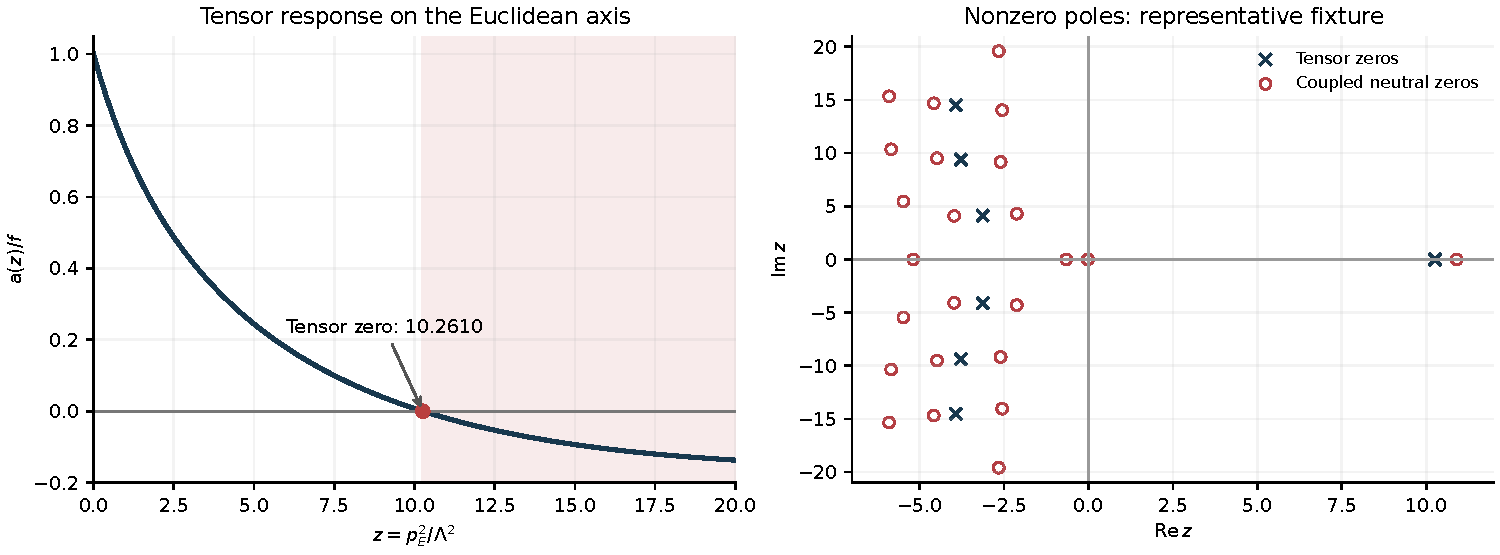
\includegraphics[width=\linewidth]{images/finite_momentum_poles.pdf}
\caption{Representative minus profile, $\epsilon=0.01$. Left: tensor factor $\mathsf a(z)/f$ on the positive Euclidean axis, crossing zero at $z\simeq10.2610$. Right: nonzero tensor and coupled neutral zeros inside the declared complex search square; conjugates are included. Closely spaced roots and the light poles near the origin overlap at this scale. The map is a bounded numerical result, not a physical particle spectrum.}
\end{figure}

Complex poles and negative-residue tachyons obstruct an ordinary positive spectral interpretation under the tested prescription. No claim is made that an unspecified nonstandard contour repairs them. Nor does this calculation prove the impossibility of every modified action or completion of the broader research program.
